\title{ALPS Application Tutorial}

\begin{document}

\lstset{language={C++},showspaces=false,rulecolor=\color[cmyk]{0, 0.29,0.84,0}}

\begin{frame}
  \titlepage
\end{frame}

\section*{Outline}
\begin{frame}
   \tableofcontents
\end{frame}

\section{Workflow of ALPS Simulation / ALPSシミュレーションの流れ}
\subsection*{{\protect\color{red}●}{\protect\color{blue}●}}

\begin{frame}{Workflow of ALPS Simulation}
  \begin{center}
    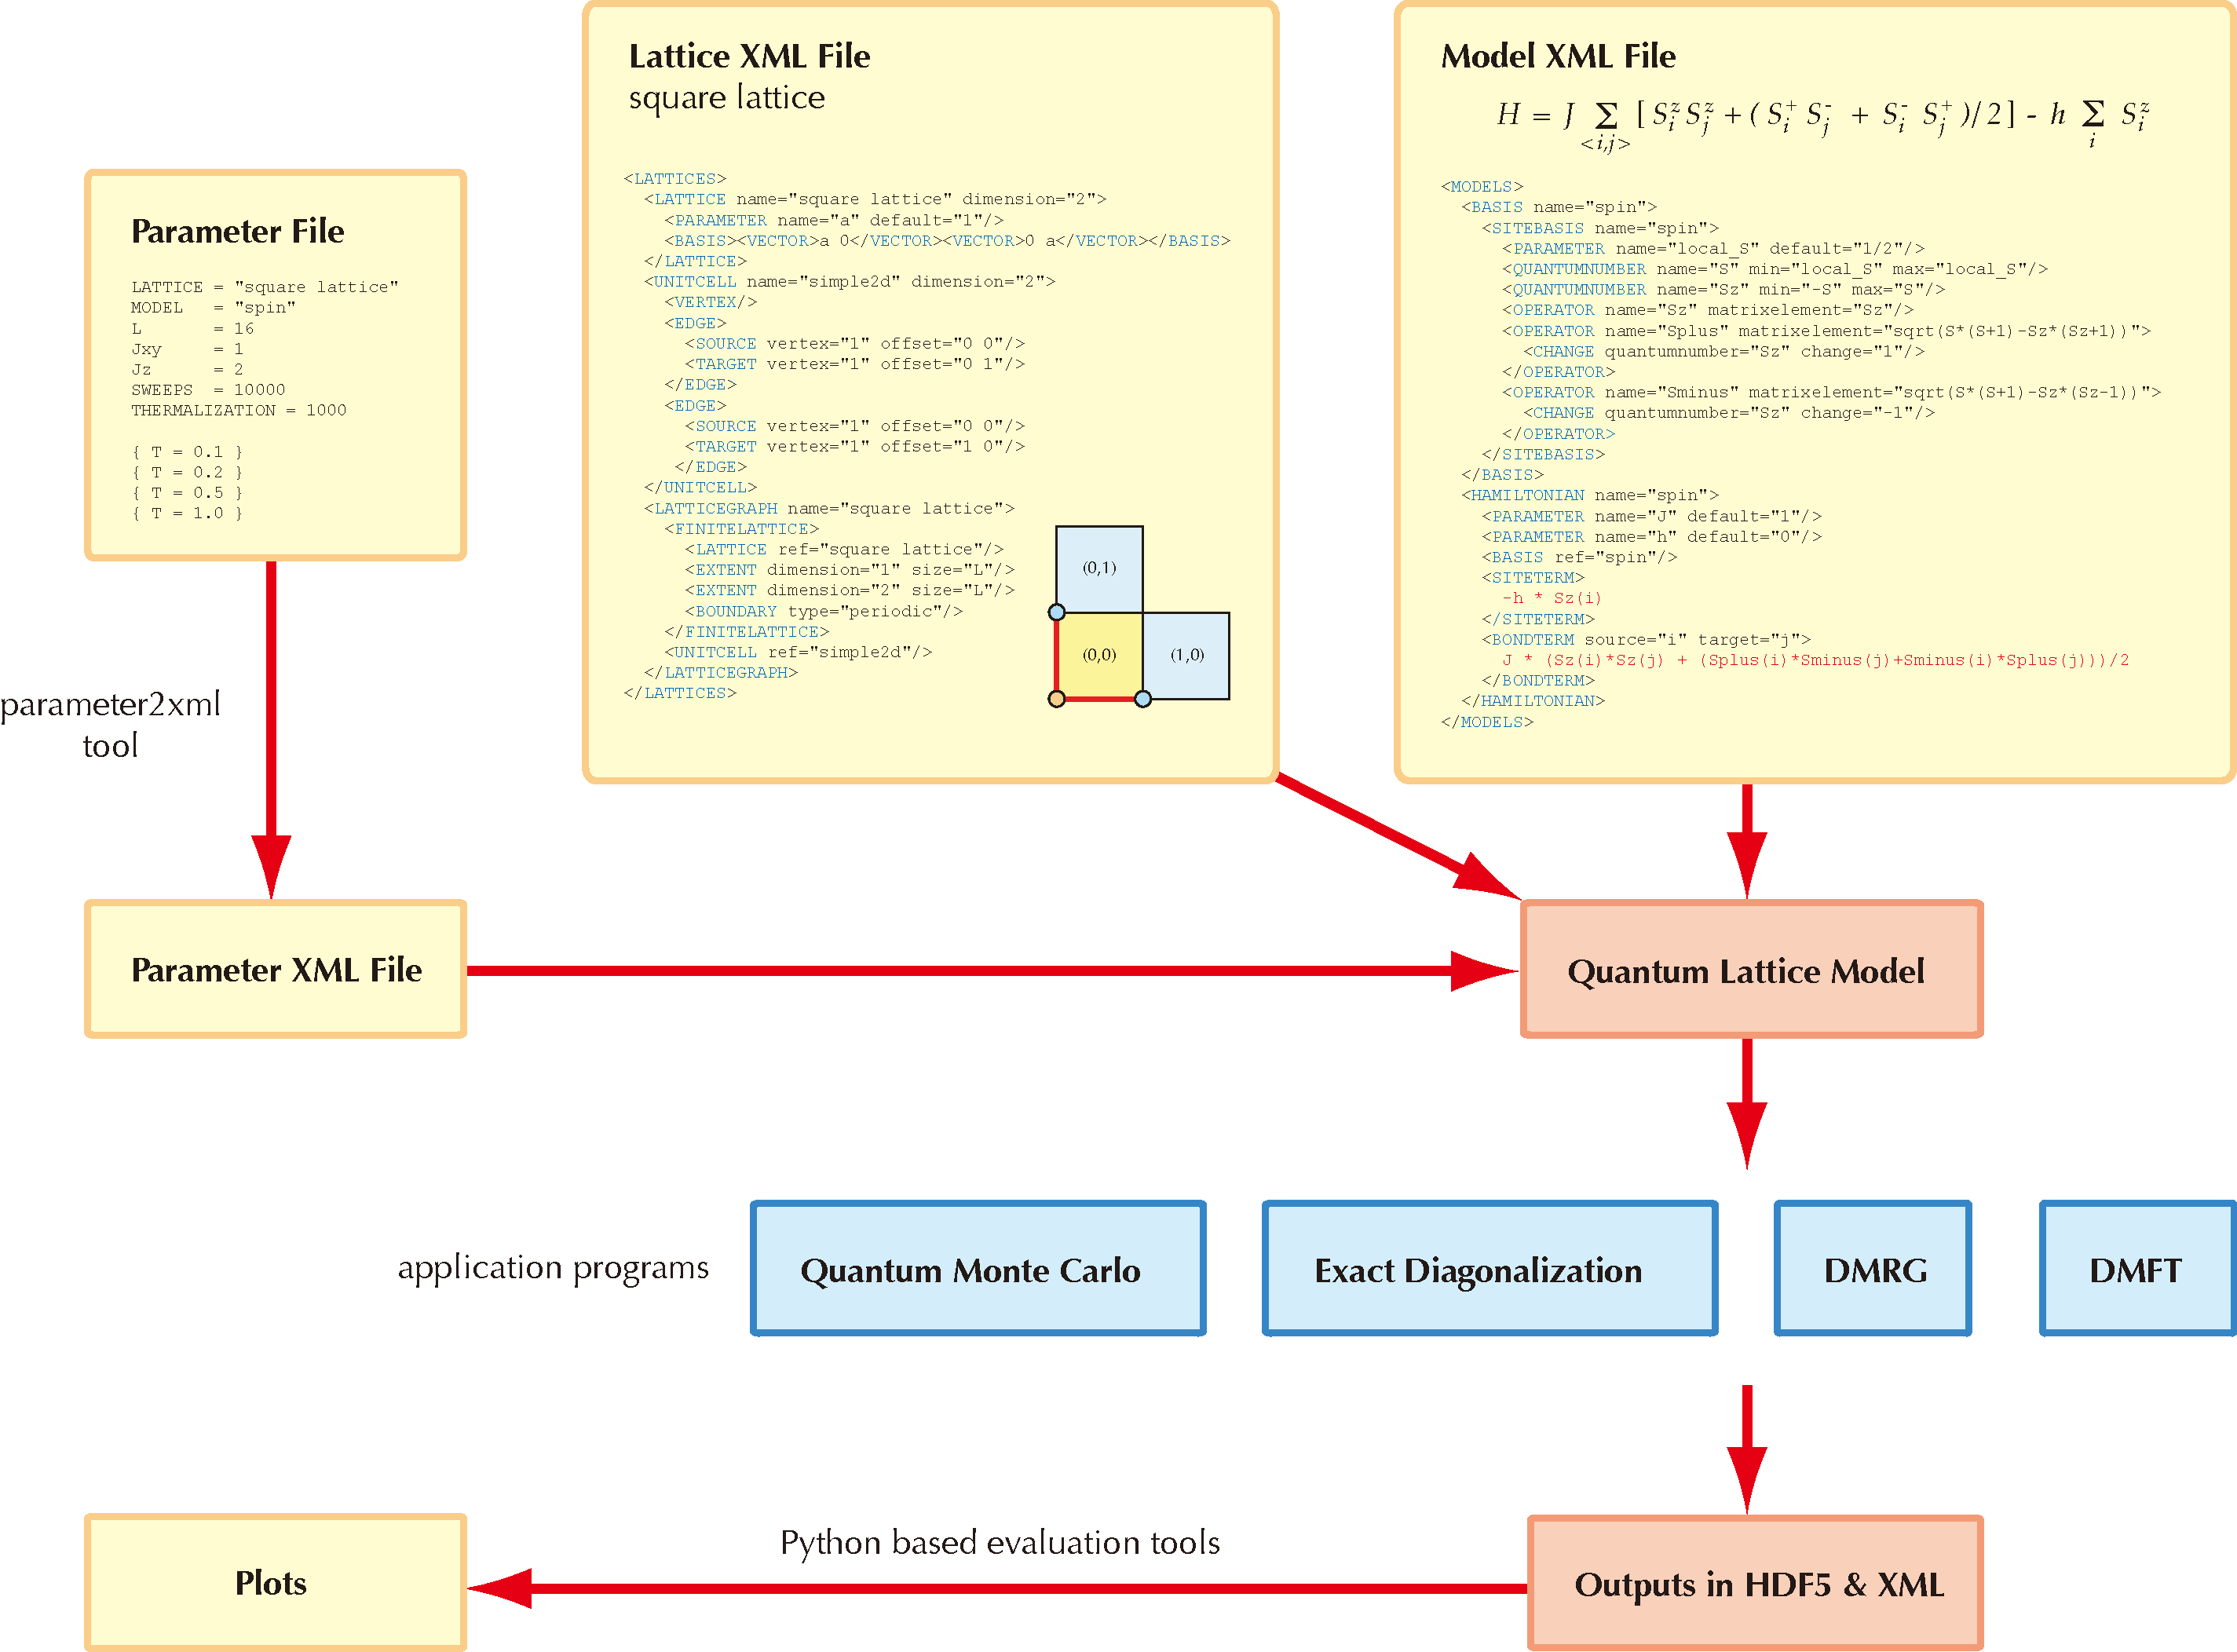
\includegraphics[height=0.8\textheight]{workflow.pdf}
  \end{center}
\end{frame}

\begin{frame}{ALPS Setup Script}
  \begin{itemize}
  \item alpsvars.sh: Shell script for setting environment variables, {\tt ALPS\_HOME}, {\tt PATH}, {\tt LD\_LIBRARY\_PATH}, {\tt PYTHONPATH}, etc
  \item on psi.issp.u-tokyo.ac.jp

    {\tt /opt/MateriApps/alps/alpsvars.sh}
  \item on phi.aics.riken.jp
    
    {\tt /home/materiapps/alps/alpsvars.sh}
  \item on kashiwa.issp.u-tokyo.ac.jp
    
    {\tt /home/issp/materiapps/alps/alpsvars.sh}
  \item on k.aics.riken.jp
    
    {\tt /opt/spire/alps/alpsvars.sh}
  \end{itemize}
  \begin{alertblock}{}
    alpsvars.sh script is provided for all the computers on which ALPS has been installed. For current status of installation, see \footnotesize \url{https://github.com/wistaria/MateriAppsInstaller}.
\end{alertblock}
\end{frame}

\begin{frame}[fragile]
  \frametitle{Preparation for Running Tutorials}
  \begin{enumerate}
  \item SSH login to workstation
\begin{semiverbatim}
\$ ssh -YC{\it hostname} -l{\it username}
\end{semiverbatim}
  \item Set up environment variables
\begin{semiverbatim}
\$ source /\!\!{\it somewhere}/alpsvars.sh
\end{semiverbatim}
  \item Check if ALPS tool works correctly or not
\begin{semiverbatim}
\$ pconfig
\end{semiverbatim}
  \item Copy tutorial files
\begin{semiverbatim}
\$ cp -rp $ALPS\_HOME/tutorials $HOME
\end{semiverbatim}
  \end{enumerate}
\end{frame}

\begin{frame}[fragile]
  \frametitle{Miki's First ALPS Simulation}
  \begin{itemize}
    \item Run simulations from python
\begin{semiverbatim}
\$ cd $HOME/tutorials/mc-02-susceptibilities
\$ python tutorial2a.py
\$ python tutorial2b.py
\$ python tutorial2c.py
\$ python tutorial2d.py
\$ python tutorial2full.py
\end{semiverbatim}
    \item Everytime you run python script, plot window will open.
    \item Python script will finish by closing plot window.
    \item The last script will show results of all the simulations in one plot.
  \end{itemize}
\end{frame}

\end{document}
